\subsection{Comparison of Young's Modulii Used in DEM Simulations}\label{sec:dem-studies-youngs-modulus}

The discrete element method is used by many ceramic breeder researchers to model the interaction of individual pebbles in an ensemble.\cite{An20071393, Lu2000, Zhao2010, Gan:2010uq, Annabattula2012a, VanLew2014} In the past studies, the Young's modulus of the ceramic materials used in DEM simulations was taken from historical data, for instance lithium metatitanate from Ref.~\cite{Gierszewski1998}. However, as discussed in \cref{sec:exp-reduction-factor}), I proposed a modification of the Young's modulus to be used in DEM simulations for a batch of ceramic pebbles based on the `softening' seen of most pebbles in experiments. The force-displacement curves of Figs~\ref{fig:fzk-exp-hertz} and~\ref{fig:nfri-exp-hertz} demonstrate how far from the ideal Hertzian curves the majority of of ceramic pebbles behave.

The Hertzian force is linearly proportional to the pair Young's modulus of contacting spheres. Based on the $\kappa$ values found in \cref{sec:exp-reduction-factor}, the apparent Young's modulii of \lis and \lit are, on average, less than half the values given for sintered materials in literature. For the case of \lit, the average value was closer to only 10\% of the value from literature. Thus the actual contact forces in pebble beds may be 10\% of the values found from DEM simulations! The contact force is a critical value for determining the conduction heat transport between pebbles as well as damage prediction. It is crucial to use proper material properties in our simulations in order to have dependable predictions of pebble crushing events. In this section, we will compare a number of pebble beds under numerical simulations of uniaxial compression tests. One set of beds will be composed of pebbles with the Young's modulus from literature and the other set will be composed of pebbles with a distribution of Young's modulus that fits the distribution from an experiment.
%~~~~~~~~~~~~~~~~~~~~~~~~~~~~~~~~~~~~~~~~~~~~~~~~~~~~~~~~~~~~~~~



%~~~~~~~~~~~~~~~~~~~~~~~~~~~~~~~~~~~~~~~~~~~~~~~~~~~~~~~~~~~~~~~
\subsubsection{Numerical Setup}
%In pebble bed breeder units, the stresses on the pebble regions are a result of thermal expansion of the relatively hot pebbles contained by relatively cool container walls. This process is a function of the coefficient of thermal expansion of the pebbles and their elevated temperature; the confined strain relates to a stress. 
The pebble beds are modeled as undergoing a standard uniaxial compression up to 6 MPa while measuring the macroscopic stress-strain for some parametrically varied pebble beds and compare the curves. At the moment of maximum stress, we can investigate the differences in contact forces of those pebble beds.

Our pebble ensemble is composed of \si{0.5 mm} diameter \lis pebbles. The pebble beds are initiated and packed in the same manner as \cref{sec:dem-studies-effective-conductivity}. There are two main bed groups. Set A: the first set of three beds (A.1-3) contain a single type of pebble with $E$ = \si{90 GPa}. Set B: the second set of four beds (B.1-4) contain ten types of pebbles with their Young's modulus assigned in a discrete, random way to satisfy the distribution seen from experimental data. For the DEM study, I fit to \lis pebbles with a Weibull distribution of shape parameter $\sigma = 1.6$ where the average stiffness was $\bar{E} = 49$~GPa. The description of the two sets of pebble beds is visually represented in Fig.~\ref{fig:dem-types}. The pebble bed geometry was also the same used in the study of Ref.~\cite{VanLew2014}; two virtual walls in the x-direction located at $x_\text{lim} = \pm 20 R_p$, periodic boundaries at the limits of $y_\text{lim} = \pm 15 R_p$, and a total of 8000 pebbles packed into the volume to an approximate height of $z_\text{lim} = 20 R_p$.

Among both sets, a parametric study was done on pebble radius and coefficient of friction. The radii of pebbles in beds A.1, A.2, B.1, and B.2 were constant at $R_p$=.25 mm. The radii of pebbles in beds A.3, B.3, and B.4 followed a Gaussian distribution about $\bar{R}_p$ = 0.25 mm: $\mu_d = R_p$ and $sigma_d = R_p$. The coefficient of friction was set at $\mu = 0.2$ for beds A.1, A.3, B.1, and B.3; the coefficient of friction was $\mu = 0.3$ for beds A.2, B.2, and B.4.


\begin{figure}[t]
  \centering
  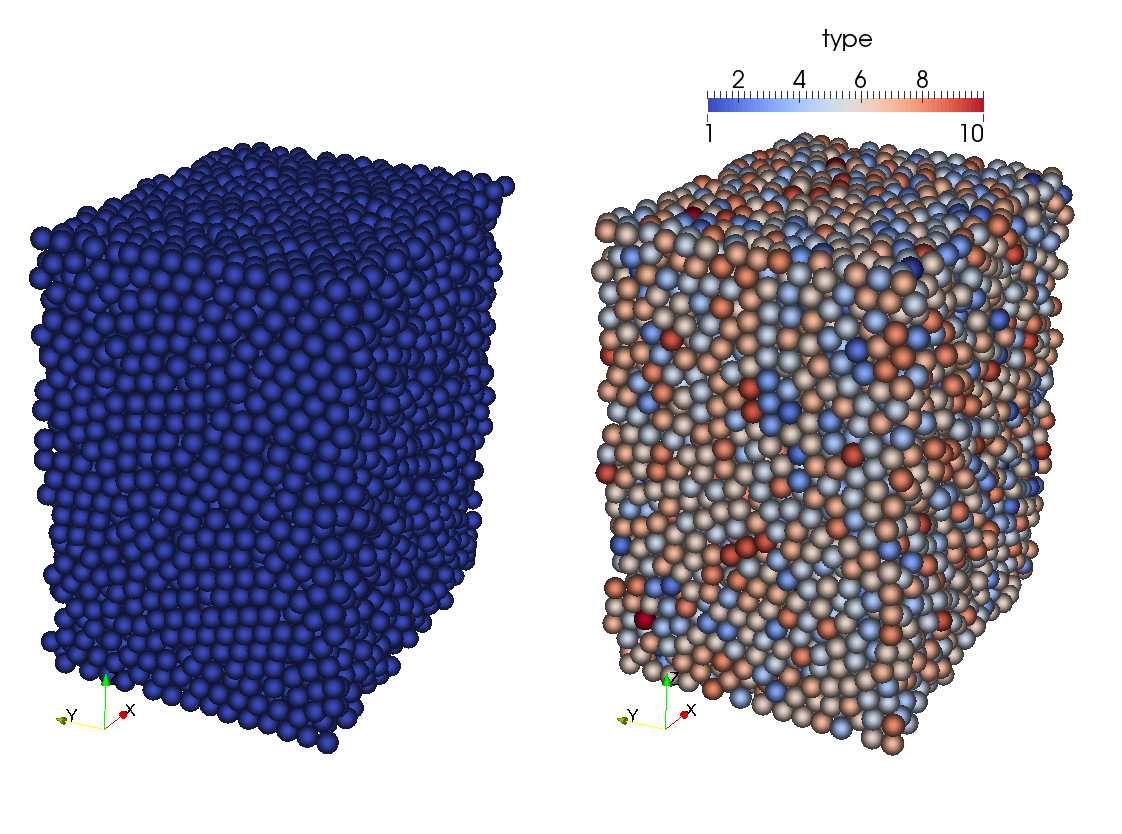
\includegraphics[width=\singleimagewidth]{chapters/figures/DEM-types}
  \caption{On the left, set A, a pebble bed with a single type, of $E = 120$ GPa. On the right, set B, is a pebble bed with 10, randomly distributed types; each type corresponds to a reduced, apparent Young's modulus as derived from experimental data.}\label{fig:dem-types}
\end{figure}
%~~~~~~~~~~~~~~~~~~~~~~~~~~~~~~~~~~~~~~~~~~~~~~~~~~~~~~~~~~~~~~~





%~~~~~~~~~~~~~~~~~~~~~~~~~~~~~~~~~~~~~~~~~~~~~~~~~~~~~~~~~~~~~~~
\subsubsection{Results from Uniaxial Compression}


A constant-velocity, uniaxial compression was applied to the pebble beds. A single cycle up to 6 MPa was used on all the beds. The macroscopic measurements of stress-strain are shown for all the pebble beds in Fig.~\ref{fig:stress-strain}.

\begin{figure}[t]
  \centering
  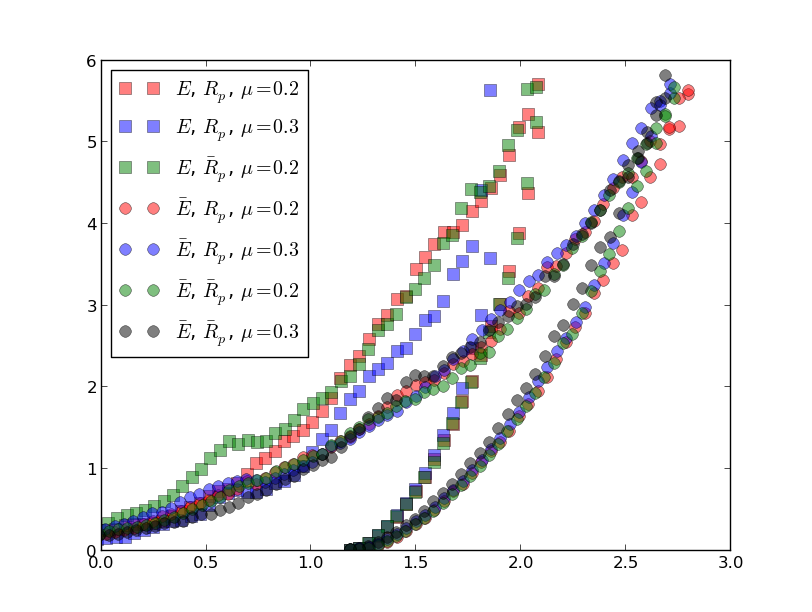
\includegraphics[width=\singleimagewidth]{chapters/figures/stress-strain}
  \caption{Stress-strain responses of pebble beds with: squares, constant Young's modulus; and circles, Gaussian distribution of Young's modulus. The constant Young's modulus beds all had much firmer responses for all parametric cases studied here.}\label{fig:stress-strain}
\end{figure}

Naturally, the pebble beds with smaller Young’s modulus (with circle markers) are more compliant to external loads. The result is true regardless of the coefficient of friction or distribution of pebble radius studied here. Group B moved to an average strain of about 2.6\% at 6 MPa, by comparison the beds of Group A only had strained 1.9 \% on average to reach the same stress. Among the beds of each group, pebble beds with constant radius pebbles behaved virtually the same as similar pebble beds with a Gaussian distribution on radius. An increase in the coefficient of friction had a moderate impact on the overall stress-strain response. 


The parametric study here shows that the largest contributor to stress-strain response is the Young’s modulus. The coefficient of friction and radius distribution had comparatively insignificant influence. A pebble bed geometry more directly comparable to oedometric compression experiments should be used to allow direct comparison and validation of the numerical models.


At the point of peak stress for each bed, I use DEM results to visualize the distribution of contact forces among all pebbles in the ensemble. A plot of the probability distributions of all the beds together, Fig.~\ref{fig:all-contact-forces}, shows that the majority of the contacts in all the beds are equally small. There are a few overall trends we observe from the results however. The pebble beds with the constant Young's modulus are always higher for their comparable version with distributed Young's modulus. For pebble beds with comparable Young's modulii and radii, higher coefficients of friction generally have higher peak contact forces. Pebble beds' radius distributions have much less impact on peak contact forces than either coefficient of friction or Young’s modulus. Another method of comparing overall contact force distributions is to consider predictions on pebble cracking which assigns a strength value at random to pebbles in the bed, according to Eq.~\ref{eq:crush-predict}. At the point of maximum stress, this is done and the results are shown in Tab.~\ref{tab:num-crush-percent}.

While overall the predicted number of broken pebbles is small, we compare similar parameteric pebble beds and in each case pebble beds with modified Young’s modulus overall predict smaller percentages of broken pebbles. Pebble crushing is a major topic for the overall evaluation of the feasibility of ceramic pebble beds in fusion reactors. This study reveals that past DEM work on pebble crushing was likely over-predicting the extent of crushing if the Young's modulus used in the study was much larger than the realistic response of individual pebbles.

\begin{figure}[t]
  \centering
  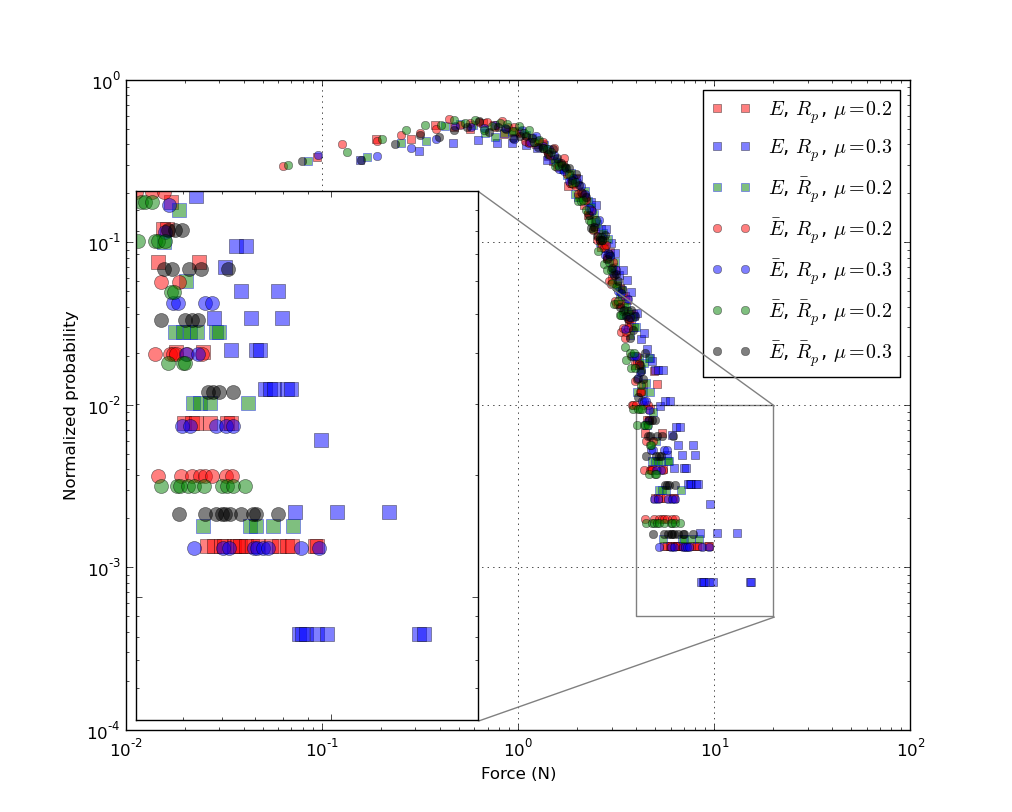
\includegraphics[width=\singleimagewidth]{chapters/figures/all-contact-forces}
  \caption{Probability distribution of contact forces in all the pebble beds studied here. Elastic moduli value is the largest contributor to higher peak contact forces among pebbles.}\label{fig:all-contact-forces}
\end{figure}


\begin{table}[t]
\caption{Comparisons for the two styles of Young's modulii used in the study. }
\label{tab:num-crush-percent}\centering
\begin{tabular}{llS[table-format=3.2]}
\toprule
Bed label		& 		Parameters 								&	\text{Predicted crushed}			\\
				& 												&	\multicolumn{1}{r}{\text{\%}}		\\\otoprule
A.1				& 		$E$, $R_p$, $\mu = 0.2$          		&	0.3									\\\midrule
A.2				& 		$E$, $R_p$, $\mu = 0.3$     			&	1.0									\\\midrule
A.3				& 		$E$, $\bar{R}_p$, $\mu = 0.2$			&	0.9									\\\midrule
B.1				& 		$\bar{E}$, $R_p$, $\mu = 0.2$			&	0.6									\\\midrule
B.2				& 		$\bar{E}$, $R_p$, $\mu = 0.3$			&	0.8									\\\midrule
B.3				& 		$\bar{E}$, $\bar{R}_p$, $\mu = 0.2$		&	0.4									\\\midrule
B.4				& 		$\bar{E}$, $\bar{R}_p$, $\mu = 0.3$		&	0.7									\\\bottomrule
\end{tabular}
\end{table}
%~~~~~~~~~~~~~~~~~~~~~~~~~~~~~~~~~~~~~~~~~~~~~~~~~~~~~~~~~~~~~~~






%~~~~~~~~~~~~~~~~~~~~~~~~~~~~~~~~~~~~~~~~~~~~~~~~~~~~~~~~~~~~~~~
\subsection{Conclusions of Young's Modulus Study}
Variation in production techniques for ceramic pebbles have lead to batches of pebbles with slight differences in their ceramic microstructure, as evident in the wide distribution of crush loads reported in past studies, \textit{e.g.} Refs.~\cite{Zhao2012,Mandal2012a}. By the same token, the different microstructures should naturally lead to variation in Young’s modulus. However up to now values of Young’s modulus used in numerical models are taken from values measured for large sintered pellets of ceramic materials. Based on single pebble experiments and the application of Hertz theory, a technique for introducing a modified Young’s modulus into DEM models has been proposed here. DEM simulations show the impact of modified pebble elasticity on both macroscopic measurements of stress-strain curves as well as mesoscopic measures of inter-pebble contact force -- with major implications for prediction of pebble crushing in ceramic pebble beds. The models applying the softening coefficient, $k$, predict more compliant pebble beds and smaller peak contact forces in beds and thus fewer crushed pebbles.

Thus we conclude that in DEM numerical models for pebble damage, the modified Young's modulus with softening coefficients matching the probability density function from experiments must be used. Experimental work has revealed pebble beds behaving with much softer elasticity coefficients than those found from sintered blocks of past studies. The inter-particle forces of the modified Young's Modulus are therefore smaller than previous predictions by the same order of magnitude as the error in elasticity coefficient. In this way, we can expect a more realistic numerical tool to simulate pebble damage, bed rearrangement, and heat transfer.